\documentclass[xcolor=table,10pt,final]{beamer}
\renewcommand\mathfamilydefault{\rmdefault}

\setbeamertemplate{navigation symbols}{}
\usepackage{amsmath,amsfonts,amssymb,pxfonts,xspace}
\usepackage{textcomp}
\usepackage{lmodern}
\usepackage{verbatim}
\usepackage{graphicx}
\usepackage{listings}
\usepackage[T1]{fontenc}


\lstset{
    language=Python,
    basicstyle=\footnotesize,
    keywordstyle=\color[rgb]{0.1,0.8,0.1}\bfseries,
    commentstyle=\color{blue},
    numbers=left,
    stringstyle=\ttfamily\color{red!50!brown},
    showstringspaces=false}
\lstset{literate=%
   *{0}{{{\color{red!20!violet}0}}}1
    {1}{{{\color{red!20!violet}1}}}1
    {2}{{{\color{red!20!violet}2}}}1
    {3}{{{\color{red!20!violet}3}}}1
    {4}{{{\color{red!20!violet}4}}}1
    {5}{{{\color{red!20!violet}5}}}1
    {6}{{{\color{red!20!violet}6}}}1
    {7}{{{\color{red!20!violet}7}}}1
    {8}{{{\color{red!20!violet}8}}}1
    {9}{{{\color{red!20!violet}9}}}1
}



\begin{document}

\title{Python for Scientific Computing}
\subtitle{Lecture 1: The Python Calculator}
\author{Albert DeFusco\\Center for Simulation and Modeling}
\date{\today}
\frame{\titlepage}

\section{Computer Programming}
\frame{\sectionpage}
\begin{frame}[fragile]
  \frametitle{} %Computer programming: Dot Product}
  {\scriptsize
  \begin{equation*}
    \mathbf{a}\cdot\mathbf{b} = \sum_{i=1}^{n}a_ib_i
  \end{equation*}
}
  \begin{columns}
    \begin{column}{0.5\paperwidth}
      \begin{block}{Assembler}
\lstset{
      basicstyle=\tiny
    }
  \begin{lstlisting}[language={[x86masm]Assembler}]
global _mult3
sum equ 16
section .text
_mult3:
  push ebp
  mov ebp,esp
  push esi
  push edi
  sub esp, 4
  mov esi, [ebp+12]
  mov edi, [ebp+8]
  mov dword [ebp-sum], 0
  mov ecx, 3
.forloop:
  mov eax, [edi]
  imul dword [esi]
  add edi, 4
  add esi, 4
  add [ebp-sum], eax
  loop .forloop
  mov eax, [ebp-sum]
  add esp, 4
  pop edi
  pop esi
  pop ebp
  ret
\end{lstlisting}
\end{block}
\end{column}
\begin{column}{0.35\paperwidth}
  \begin{block}{C source\footnotemark}
\lstset{
      basicstyle=\tiny
    }
  \begin{lstlisting}[language=C]
int mult3( int *dst, int *src)
{
  int sum = 0, i;

  for (i = 0; i < 3; i++)
    sum += dst[i] * src[i];

  return sum;
}

int main(void)
{
  int d[3] = { 1, 2, 3};
  int s[3] = {8, 9, 10 };

  printf("answer is %i\n", mult3(d, s) );
  return 0;
}
      \end{lstlisting}
    \end{block}
    \end{column}
  \end{columns}
  {\tiny \footnotetext{\tiny The first compiler was written by Grace Hopper in 1952 for the A-0 language}}
\end{frame}

\begin{frame}[fragile]
  \frametitle{} %Computer programming}
  {\scriptsize
  \begin{equation*}
    \mathbf{a}\cdot\mathbf{b} = \sum_{i=1}^{n}a_ib_i
  \end{equation*}
}
\lstset{
      basicstyle=\footnotesize
    }
  \begin{block}{Python}
    \begin{lstlisting}[language=Python]
import numpy
dist = numpy.array([1,2,3])
src  = numpy.array([8,9,10])

print dist.dot(src)
\end{lstlisting}
\end{block}
\end{frame}

\begin{frame}
  \frametitle{Choices}
  \begin{columns}[c]
    \begin{column}{0.4\paperwidth}
      \begin{block}{Computer Time}
        %\begin{itemize}
        %  \item Interpret Python and run
        %\end{itemize}
      \end{block}
    \end{column}
    \begin{column}{0.4\paperwidth}
      \begin{block}{Programmer Time}
        %\begin{itemize}
        %  \item Write and Debug compiled code
        %\end{itemize}
      \end{block}
    \end{column}
  \end{columns}
\end{frame}


\begin{frame}
  \frametitle{History of Python}
  \begin{itemize}
    \item December 1989
      \begin{itemize}
        \item Implementation by Guido van Rossum as successor of ABC to provide exception handling
      \end{itemize}
    \item February 1991
      \begin{itemize}
        \item Python 0.9.0 had classes with inheritance, exception handling, functions, and the core datatypes
      \end{itemize}
    \item January 1994
      \begin{itemize}
        \item Version 1.0 has functional programming features
      \end{itemize}
    \item October 2000
      \begin{itemize}
        \item Python 2.0 brings garbage collections
        \item Python 2.2 improves Python's types to be purely object oriented
      \end{itemize}
    \item December 2008
      \begin{itemize}
        \item Python 3
        \item {\it Reduce feature duplication by removing old ways of doing things}
        \item Not backwards compatible with Python 2.x
      \end{itemize}
  \end{itemize}
\end{frame}

\begin{frame}
  \frametitle{What's so great about Python?}
  \begin{itemize}
    \item Portable
      \begin{itemize}
        \item Your program will run if the interpreter works and the modules are installed
      \end{itemize}
  \end{itemize}
\end{frame}
\begin{frame}
  \frametitle{What's so great about Python?}
  \begin{itemize}
    \item Efficient
      \begin{itemize}
        \item Rich language features built in
        \item Simple syntax for ease of reading
        \item Focus shifts to ``algorithm'' and away from implementation
      \end{itemize}
  \end{itemize}
\end{frame}
\begin{frame}
  \frametitle{What's so great about Python?}
  \begin{itemize}
    \item Flexible
      \begin{itemize}
        \item Imperative
        \item Object-oriented
        \item Functional
      \end{itemize}
  \end{itemize}
\end{frame}
\begin{frame}
  \frametitle{What's so great about Python?}
  \begin{itemize}
    \item Extendible
      \begin{itemize}
        \item Plenty of easy-to-use modules
          \begin{itemize}
            \item {\it If you can imagine it, then someone has probably developed a module for it}
          \end{itemize}
        %\item separate the interface from the implementation
        \item Your program can adjust the way the interpreter works
      \end{itemize}
  \end{itemize}
\end{frame}

\begin{frame}
  \frametitle{Why use python for science?}
  \begin{itemize}
    \item A highly programmable calculator
    \item Fast proto-typing new algorithms or program design
    %\item Can create an easily programmable interface to many more complex programs
    \item Use C or Fortran routines directly
    \item Many science and mathematics modules already exist
  \end{itemize}
\end{frame}

\begin{frame}[fragile]
  \frametitle{Development Environment}
  \begin{columns}
    \begin{column}{0.5\paperwidth}
      \begin{itemize}
        \item Frank
          \begin{enumerate}
            \item Launch Putty
            \item Connect to {\tt login0a.frank.sam.pitt.edu}
          \end{enumerate}
      \end{itemize}
    \end{column}
    \begin{column}{0.5\paperwidth}
      \centering
      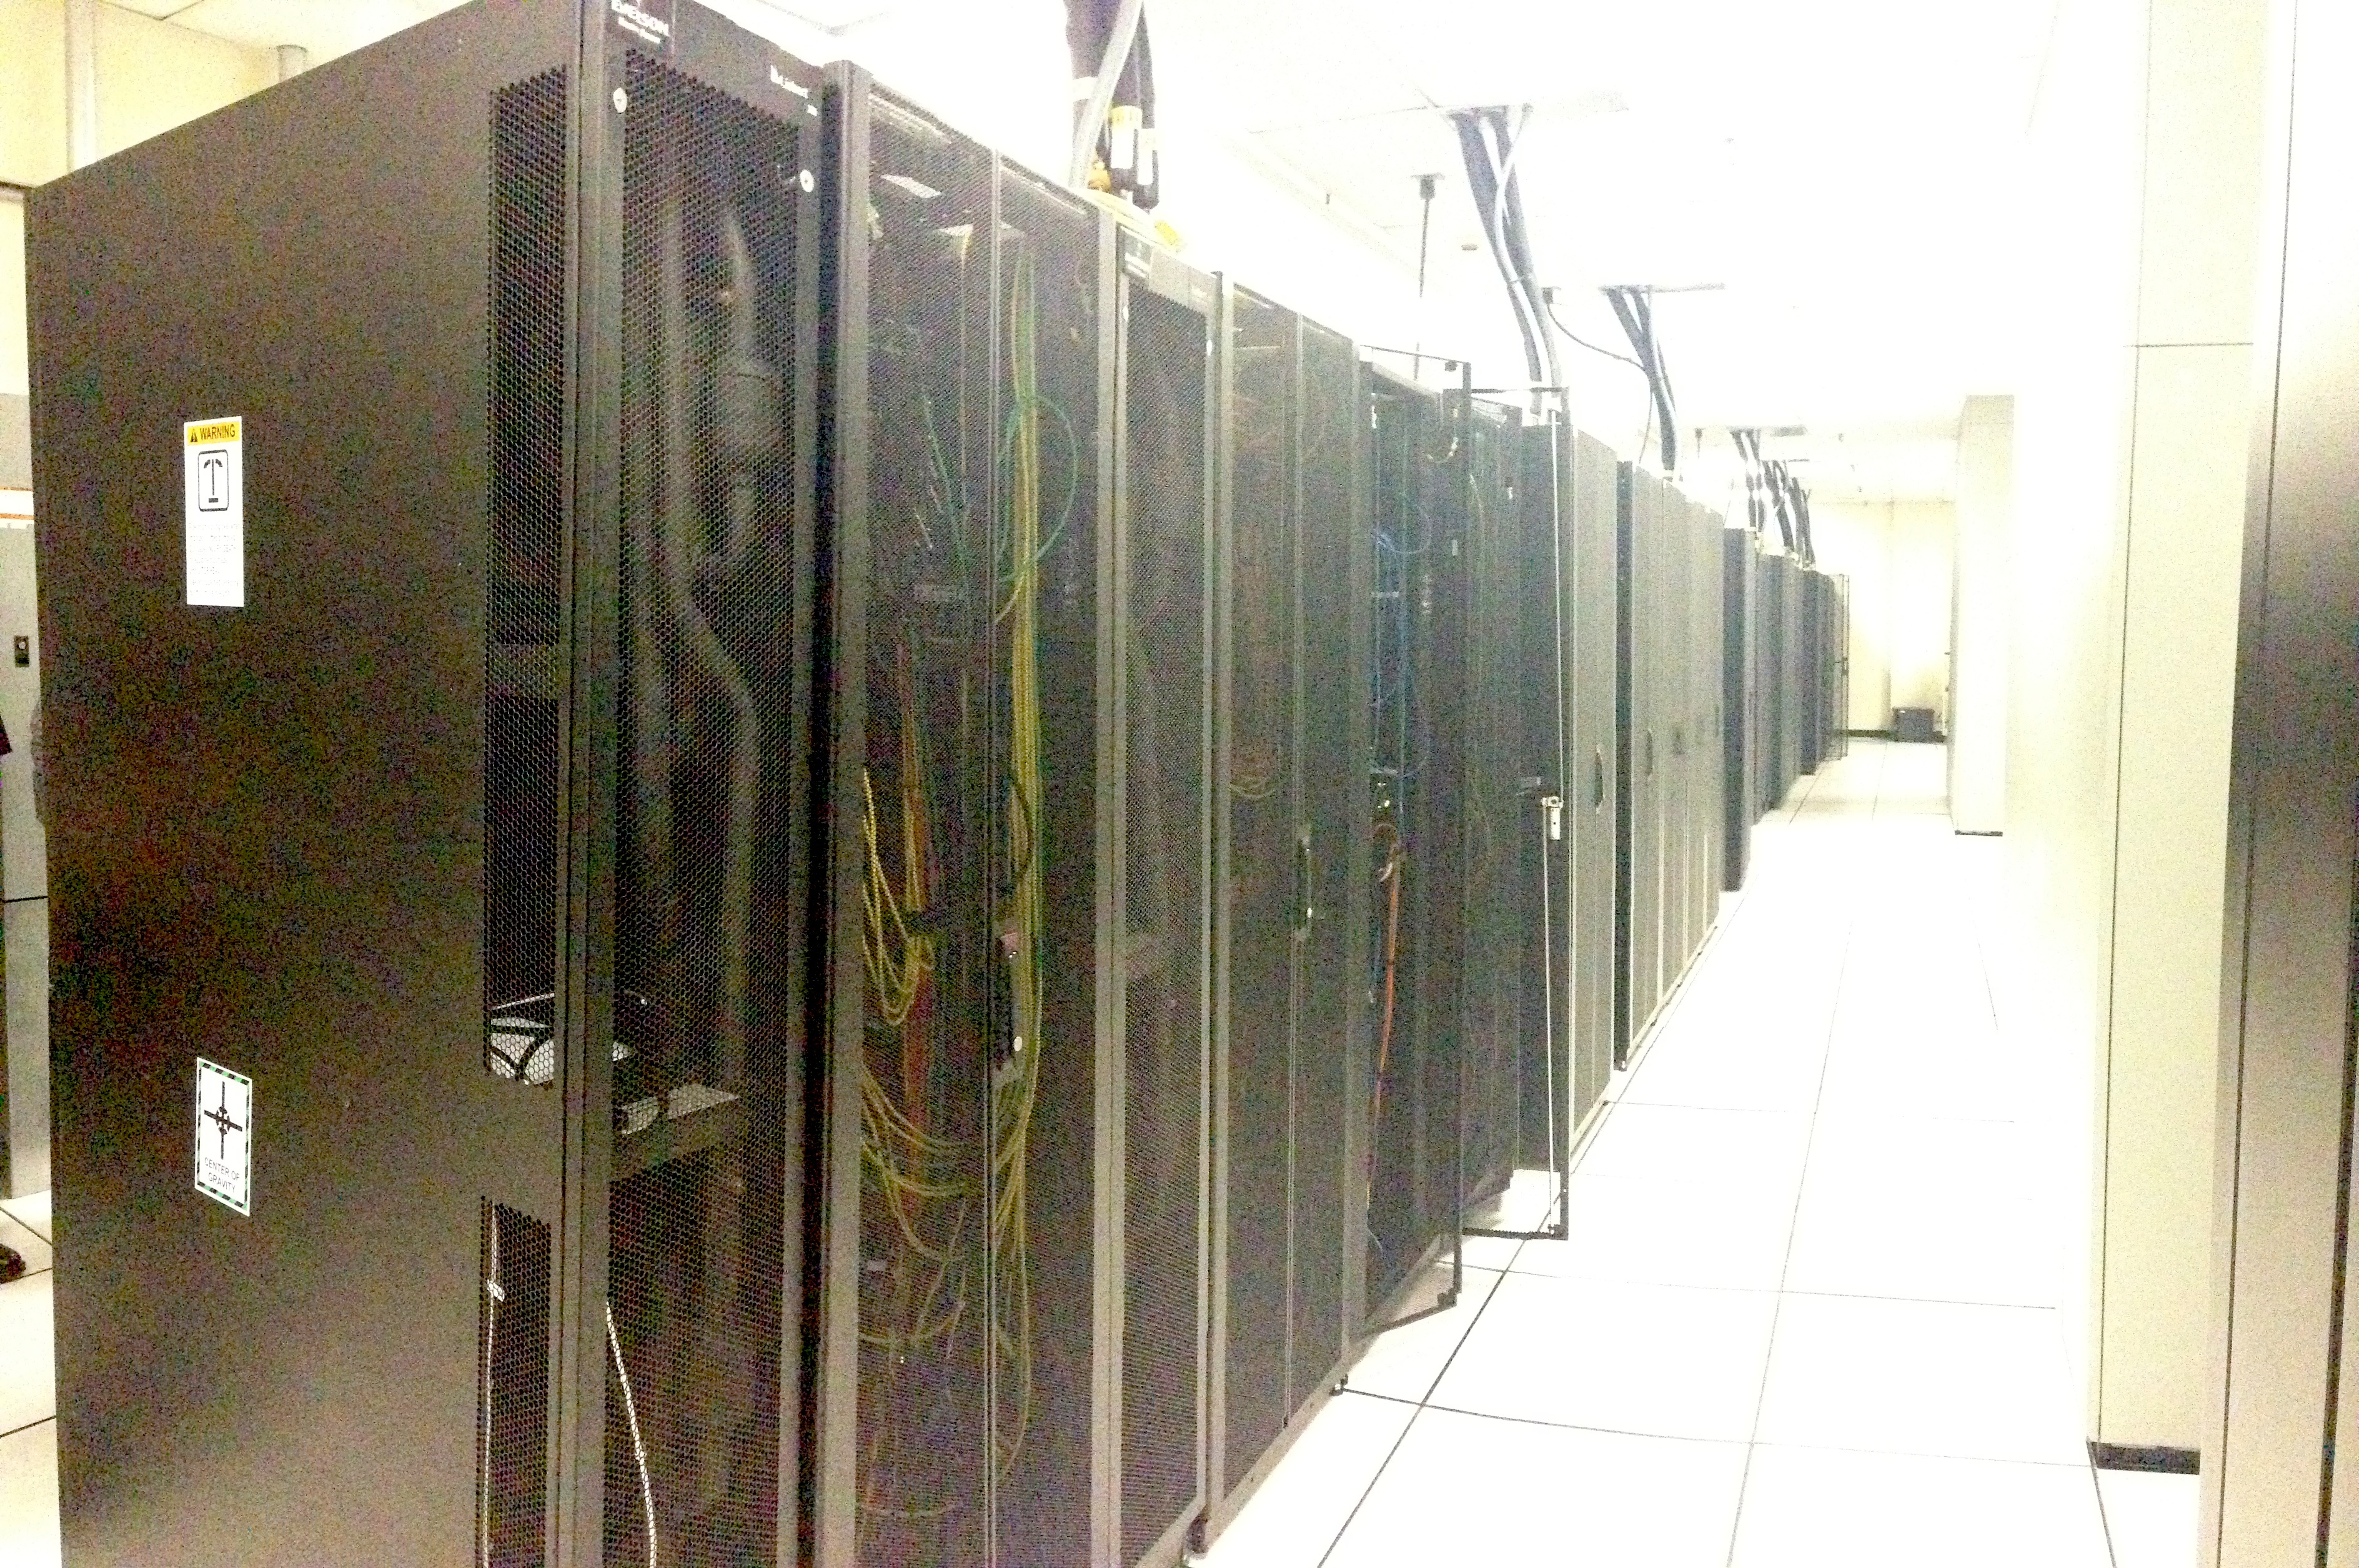
\includegraphics[width=0.48\paperwidth]{figures/frank}
    \end{column}
  \end{columns}
\end{frame}

\begin{frame}[fragile]
  \frametitle{Read the documentation}
  \begin{verbatim}
> pydoc

> python
>>> help()
\end{verbatim}
\end{frame}

\begin{frame}[fragile]
  \frametitle{Disclaimer}
  Python 2.7 $!=$ 3.0
  \vskip1cm
  \begin{verbatim}
http://wiki.python.org/moin/Python2orPython3
\end{verbatim}
\end{frame}

\begin{frame}
  \frametitle{Python syntax}
  \begin{itemize}
    \item Extremely simplified syntax
      \begin{itemize}
        \item Nearly devoid of special characters
        \item Intended to be nearly English
      \end{itemize}
    \item Dynamic types
      \begin{itemize}
        \item It is the responsibility of the programmer
        \item Still ``strongly typed''
      \end{itemize}
  \end{itemize}
\end{frame}

\begin{frame}[fragile]
  \frametitle{Python objects}
  \begin{itemize}
    \item All data in Python is represented by objects
    \item Objects have
      \begin{itemize}
        \item an identity
        \item a type
        \item a value
        \item a name (``variable'')\footnotemark
      \end{itemize}
    \item Variables are names assigned to {\tt objects}
  \end{itemize}
  {\tiny \footnotetext{\url{http://python.net/~goodger/projects/pycon/2007/idiomatic/handout.html\#other-languages-have-variables}}}
\end{frame}

\section{Hands-on Python}
\frame{\sectionpage}

\begin{frame}[fragile]
  \frametitle{Numerical objects}
  \begin{itemize}
    \item Integers
      \begin{itemize}
        \item \lstinline[language=Python]|a = 1|
      \end{itemize}
    \item Floats
      \begin{itemize}
        \item \lstinline[language=Python]|a = 1.0|
        %\item {\tt numpy} provides precision control
      \end{itemize}
    \item Complex numbers
      \begin{itemize}
        \item \lstinline[language=Python]|a = 1.5 + 0.5j|
        \item \lstinline[language=Python]|a.real| and \lstinline[language=Python]|a.imag| return each component
      \end{itemize}
    \item Type casts
      \begin{itemize}
        \item \lstinline[language=Python]|myFloat = float(myInteger)|
        \item \lstinline[language=Python]|myInt = int(myFloat)|
      \end{itemize}
    \item Operators
      \begin{itemize}
        \item Addition \lstinline[language=Python]|+|
        \item Subtraction \lstinline[language=Python]|-|
        \item Multiplication \lstinline[language=Python]|*|
        \item Exponentiation \lstinline[language=Python]|**|
        \item Division \lstinline[language=Python]|/|
        \item Modulus \lstinline[language=Python]|%|
      \end{itemize}
  \end{itemize}
\end{frame}

\begin{frame}[fragile]
  \frametitle{Mathematical functions}
  \begin{itemize}
    \item many functions exist with the {\tt math} module
  \end{itemize}
  \begin{lstlisting}[language=Python]
import math

help(math)

print math.cos(0)
print math.pi
\end{lstlisting}
\end{frame}

\begin{frame}
  \frametitle{Logicals}
  \begin{itemize}
    \item Boolean type
      \begin{itemize}
        \item \lstinline[language=Python]|a = (3 > 4)|
      \end{itemize}
    \item Comparisons
      \begin{itemize}
        \item \lstinline[language=Python]|==|
        \item \lstinline[language=Python]|!=,<>|
        \item \lstinline[language=Python]|>|
        \item \lstinline[language=Python]|<|
        \item \lstinline[language=Python]|<=|
        \item \lstinline[language=Python]|>=|
      \end{itemize}
  \end{itemize}
\end{frame}



\begin{frame}[fragile]
  \frametitle{Strings}
  \begin{itemize}
    \item \lstinline[language=Python]|a = 'single quoted'|
    \item \lstinline[language=Python]|a = "double quoted"|
    \item Triple quotes preserve whitespace and newlines
  \end{itemize}
      \begin{lstlisting}[language=Python]
      a = """triple
      quoted
      string"""
      \end{lstlisting}
      \begin{itemize}
    \item ``\symbol{92}'' is the escape character
  \end{itemize}
\end{frame}

\begin{frame}
  \frametitle{String operations}
  \begin{itemize}
    \item Typecasting
      \begin{itemize}
        \item \lstinline[language=Python]|doubleA = float(a)|
        \item \lstinline[language=Python]|intA = int(a)|
      \end{itemize}
    \item Comparisons return a Boolean
      \begin{itemize}
        \item \lstinline[language=Python]|A == B|
      \end{itemize}
    \item \lstinline[language=Python]|concatenated = a + b|
    %\item \lstinline[language=Python]|wordList = a.split()|
  \end{itemize}
\end{frame}

\begin{frame}[fragile]
  \frametitle{Formatted strings}
  \begin{itemize}
    \item width placeholders
      \begin{table}
        \begin{tabular}{cl}
          \lstinline[language=Python]|\%s| & string\\
          \lstinline[language=Python]|\%d| & integer\\
          \lstinline[language=Python]|\%f| & float with 6 decimals\\
          \lstinline[language=Python]|\%E| & scientific notation\\
          \lstinline[language=Python]|\%\%| & the \% sign
        \end{tabular}
      \end{table}
    \item modifiers
      \begin{itemize}
        \item integers after \% adjust with width to print
        \item decimal points are specified after the width as ``.x''
        \item use a hyphen after \% to left justify
        \item printing long strings or large numbers will skew columns
      \end{itemize}
  \end{itemize}
  \begin{lstlisting}[language=Python]
from math import pi,e

print "pi is %d and e is %d" % (pi,e)
print "pi is %6.4f and e is %6.4f" % (pi,e)
print "pi is %f and e is %f" % (pi,e)
print "pi is %10.8e and e is %10.8e" % (pi,e)
print "pi is %15.8e and e is %15.8e" % (pi,e)
\end{lstlisting}
\end{frame}

\begin{frame}[fragile]
  \frametitle{Writing a script file}
  \begin{itemize}
    \item save the file to {\tt hello.py}
  \end{itemize}
\begin{lstlisting}[language=Python]
#/usr/bin/env python

#This is my comment about the following script
print 'Hello, world!'
\end{lstlisting}
\begin{itemize}
  \item run the file
\end{itemize}
\begin{verbatim}
> module load python/epd-7.2
> python hello.py
Hello, world!
\end{verbatim}
\end{frame}

\begin{frame}[fragile]
  \frametitle{Structured blocks}
  \begin{lstlisting}[language=Python]
if (a>b):
  print 'a is bigger'
else if (b>a):
  print 'big is bigger'
else
  print 'a must equal b'
\end{lstlisting}
\begin{itemize}
  \item<2-> Why is it indented?
\end{itemize}
\end{frame}
\begin{frame}
  \frametitle{Logical operations}
  \begin{itemize}
    \item \lstinline[language=Python]|not|, \lstinline[language=Python]|and|, \lstinline[language=Python]|or|
    \item be careful with assignments
      \begin{itemize}
        \item Just use if statements
      \end{itemize}
  \end{itemize}
\end{frame}

\begin{frame}[fragile]
  \frametitle{Structured blocks}
  \begin{lstlisting}[language=Python]
i=0
while (i<10):
  print i
  i=i+1
\end{lstlisting}
\end{frame}

\begin{frame}[fragile]
  \frametitle{Structured blocks}
  \begin{lstlisting}[language=Python]
for i in range(4):
  print i
\end{lstlisting}
\begin{itemize}
  \item \lstinline[language=Python]|for| is not limited to arithmetic
\end{itemize}
\end{frame}

\begin{frame}[fragile]
  \frametitle{Simple loops}
  \begin{itemize}
    \item \lstinline[language=Python]|range(start,stop,step)|
      \begin{itemize}
        \item list of integers from start to stop-1 in step increments
        \item End point is always omitted
      \end{itemize}
  \end{itemize}
\begin{lstlisting}[language=Python]
for i in range(4):
  print i
\end{lstlisting}
\end{frame}

\begin{frame}[fragile]
  \frametitle{Simple Functions}
  \begin{itemize}
    \item Simplify your program
    \item Easier debugging
    \item Improved elegance
  \end{itemize}
\begin{lstlisting}[language=Python]
import math
def area(radius):
  return math.pi*radius**2
\end{lstlisting}
\end{frame}

\begin{frame}[fragile]
  \frametitle{Simple Functions}
  \begin{itemize}
    \item Functions must be defined before being used
    \item Arguments are passed by {\it reference to the object}\footnotemark
      \begin{itemize}
        \item Variables do not have values, objects do
      \end{itemize}
    \item Functions are first class citizens
  \end{itemize}
\begin{lstlisting}[language=Python]

def y(x):
  x=x+1
  return x**2

x=5
y(x)
print x
\end{lstlisting}
{\tiny \footnotetext{\url{http://me.veekun.com/blog/2012/05/23/python-faq-passing/}}}
\end{frame}

\begin{frame}
  \frametitle{Mathematical Exercises}
  \begin{itemize}
    \item Print a table of temperature conversion
  \end{itemize}
  \vskip1cm
  \begin{equation*}
    C = \frac{5}{9}\left(F - 32\right)
  \end{equation*}
  \begin{itemize}
    \item Compute Pi using the Wallis formula
  \end{itemize}
  \vskip1cm
  \begin{equation*}
    \pi = 2\prod^{\infty}_{i=1}\frac{4i^2}{4i^2-1}
  \end{equation*}
\end{frame}


\end{document}
